\documentclass[english,serif,mathserif,xcolor=pdftex,dvipsnames,table]{beamer}
\usetheme{gc3}

\usepackage[T1]{fontenc}
\usepackage[utf8]{inputenc}
\usepackage{babel}

\usepackage{gc3}

\title[Dynamic Sequences]{%
  Dynamic and Unbounded Sequences of Tasks
}
\author[R. Murri, S3IT UZH]{%
  Riccardo Murri \texttt{<riccardo.murri@uzh.ch>}
  \\[1ex]
  \emph{S3IT: Services and Support for Science IT}
  \\[1ex]
  University of Zurich
}
\date{November~14--17, 2016}

\begin{document}

% title frame
\maketitle


\begin{frame}
  \frametitle{The \emph{3n+1} conjecture, a fictitious use case}
  \label{sec:7a}

  \+
  \begin{columns}[c]
    \column{0.5\linewidth}
    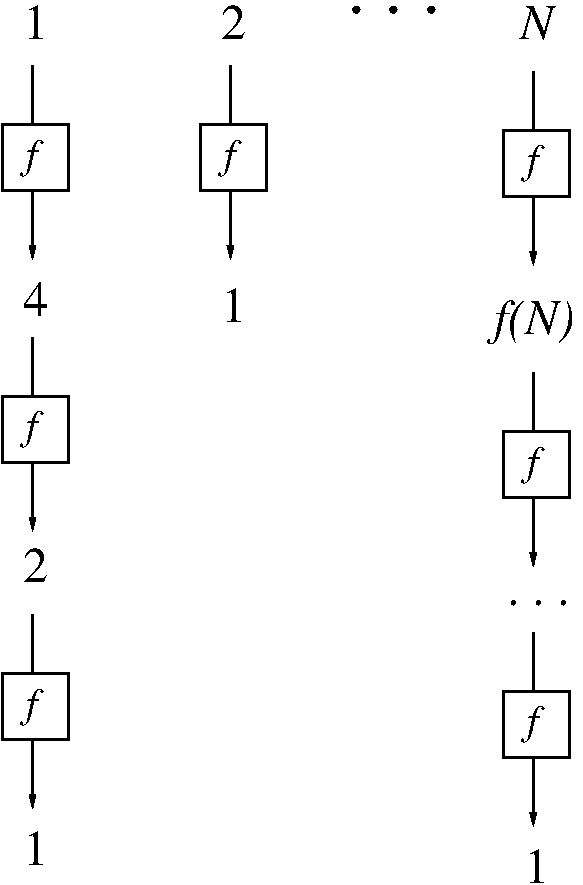
\includegraphics[height=0.8\textheight]{fig/3n+1}

    \column{0.5\linewidth}
    Define a function $f$, for $n$ positive integer:
    \begin{itemize}
    \item if $n$ is even, then $f(n) = n / 2$,
    \item if $n$ is odd, then $f(n) = 3n+1$,
    \end{itemize}

    \+
    For every positive integer $n$, form the sequence $S(n)$:
    $n \to f(n) \to f(f(n)) \to f(f(f(n))) \to \ldots$

    \+
    \textbf{Conjecture:} For every positive integer $n$, the sequence $S(n)$
    eventually hits $1$.
  \end{columns}
\end{frame}

\begin{frame}
  \frametitle{The \emph{3n+1} conjecture, \emph{(I)}}
  \label{sec:7}

  \+
  \begin{columns}[c]
    \column{0.5\linewidth}
    \includegraphics[height=0.8\textheight]{fig/3n+1_A}

    \column{0.5\linewidth}
    A computational job $F(n,k)$, applies
    function $f$ to the result of $F(n,k-1)$.

    \+
    (With $F(n,0) = n$.)
  \end{columns}
\end{frame}

\begin{frame}
  \frametitle{The \emph{3n+1} conjecture, \emph{(II)}}
  \label{sec:7b}

  \+
  \begin{columns}[c]
    \column{0.5\linewidth}
    \includegraphics[height=0.8\textheight]{fig/3n+1_S}

    \column{0.5\linewidth} 
    A sequence $H(n)$ of jobs computes the
    chain $n \to f(n) \to ... \to 1$.
  \end{columns}
\end{frame}

\begin{frame}
  \frametitle{The \emph{3n+1} conjecture, \emph{(III)}}
  \label{sec:7c}

  \+
  \begin{columns}[c]
    \column{0.5\linewidth}
    \includegraphics[height=0.8\textheight]{fig/3n+1_P}

    \column{0.5\linewidth}
    Run one sequence $H(n)$ per each $n = 1, \ldots, N$.

    \+
    They all can run in \textbf{parallel}.
  \end{columns}
\end{frame}

\begin{frame}[fragile]
  \frametitle{The \emph{3n+1} conjecture (IV)}
  \label{sec:10}

  \begin{columns}
    \column{0.25\linewidth}
    \begin{center}
      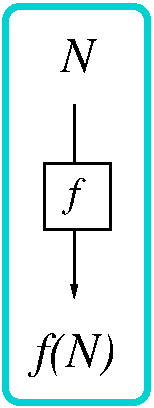
\includegraphics[height=0.8\textheight]{fig/A}
    \end{center}

    \column{0.75\linewidth}
    Let's define the simple application that computes~$f$:
    \begin{lstlisting}
class HotpoApplication(Application):
  def __init__(self, n):
    Application.__init__(
      self,
      arguments = (['/usr/bin/expr'] +
        # run `expr n / 2` if n even
        [n, '/', n] if n % 2 == 0
        # `expr 1 + 3 * n` if n odd
        else [1, '+', 3, '*', n]),
      stdout = "stdout.txt",
      # ...
    )
    \end{lstlisting}
  \end{columns}
\end{frame}

\begin{frame}[fragile]
  \frametitle{The \emph{3n+1} conjecture (V)}
  \label{sec:14}

  \begin{columns}
    \column{0.2\linewidth}
    \begin{center}
      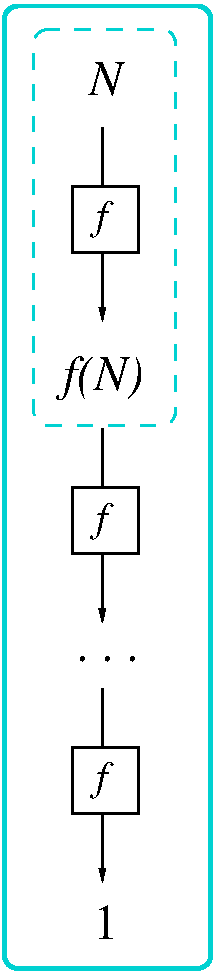
\includegraphics[height=0.8\textheight]{fig/S}
    \end{center}

    \column{0.8\linewidth}
    \small
    Now string together applications to compute a
    single sequence:
    \begin{lstlisting}[basicstyle=\ttfamily\footnotesize]
from gc3libs.workflow \
  import SequentialTaskCollection as Seq

class HotpoSequence(Seq):

  def __init__(self, n):
    # compute first iteration of $f$
    SequentialTask.__init__(self,
      [ HotpoApplication(n) ])
  
  def next(self, k):
    last = self.tasks[k].result
    if last == 1:
      return TERMINATED
    else:
      self.tasks.append(HotpoApplication(last))
      return RUNNING
    \end{lstlisting}
  \end{columns}
\end{frame}

\begin{frame}[fragile]
  \frametitle{The \emph{3n+1} conjecture (VI)}
  \label{sec:15}

  \begin{columns}
    \column{0.5\linewidth}
    \begin{center}
      \includegraphics[height=0.8\textheight]{fig/3n+1_P}
    \end{center}

    \column{0.5\linewidth}
    \small
    Parallel tasks are independent by definition, so it's even easier to
    create a collection:
    \begin{lstlisting}
tasks = ParallelTaskCollection([
  HotpoSequence(n)
  for n in range(1, N) 
])
    \end{lstlisting}

    We can run such a collection like any other \texttt{Task}.
  \end{columns}
\end{frame}


\begin{frame}[fragile]
  \begin{exercise*}[11.A]

    \+
    Fill in the missing parts and write a \texttt{hotpo.py} session-based script that:
    \begin{itemize}
    \item takes a single integer parameter $N$ on the command-line:
      \begin{semiverbatim}
\$ python hotpo.py 42        
      \end{semiverbatim}
    \item computes all the ``$3n+1$'' sequences of numbers $1$ up to $N$ in parallel,
    \item prints a final statement that the Collatz conjecture is verified up to $N$ (or ---who knows--- not?)
    \end{itemize}
  \end{exercise*}
\end{frame}


\end{document}

%%% Local Variables:
%%% mode: latex
%%% TeX-master: t
%%% End:
